\subsubsection{Long-Short Term Memory based models} \label{subsub:lstm}
The second method and the most commonly used in the Time-series Machine learning model is the Long Short-Term Memory Cell~\cite{LSTM_Hochreiter1997}.
Similar to GRU, LSTM models tend to preserve long-term dependencies in the extended data sequences.
For a longer existence, it became the most widely used type of RNN, used in those types of applications.
Figure~\ref{fig:LSTM-cell} summarises the internal cell logic.
%Currently, the most common usage of the Time-series Machine LEarning model is the prediction of stock prices, weather prognosition or any other time dependant data.
%However, the most common problem for any of those scenarios is vanishing gradient.
%Long range data tend to fade away from the model, which impacts overall prediction.
\begin{figure}[ht]%[htbp]
    \centering
    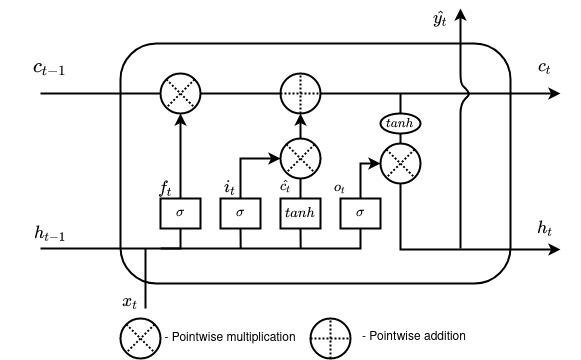
\includegraphics[width=0.7\linewidth]{II_Body/LSTM/images/LSTM.jpg}
    \caption{Long Short-Term Memory Cell}
    \label{fig:LSTM-cell}
\end{figure}
Unlike GRU, this cell utilises three gates instead of 2.
The update gate gets replaced with separate input $i_t$ and output $o_t$, as per equation~\ref{eq:LSTM-gates}.
All gets utilise the same sigmoid equation~\ref{eq:sigmoid}.
%\textcolor{red}{Those are clasical LSTM approaches. Using history sizes, no Stateless methods.}
%Unlike with GRU, the update gates renamed as an input gate $i_t$, with the same equation. Even that the forget gate $f_t$ is the same, model utilises another one, output gate $g_t$ as per Equations~\ref{eq:LSTM-gates}.
\begin{equation}
    \begin{split}
        f_t &= \sigma \left(W_f \left[h_{t-1}, x_t \right] + b_f \right) \\
        i_t &= \sigma \left(W_i \left[h_{t-1}, x_t \right] + b_i \right) \\
        o_t &= \sigma \left(W_o \left[h_{t-1}, x_t \right] + b_o \right) \\    
    \end{split}
    \label{eq:LSTM-gates}
\end{equation}
The main difference between LSTM and GRU lies in the cell state calculation.
Using the same $tanh$ activation function, Equation~\ref{eq:LSTM-output} describes how cells will be updated and propagated further.
The $c_t$ represents the cell state at a timestamp.
\begin{equation}
    \begin{split}
        \hat{c_t} &= tanh \left(W_c \left[h_{t-1}, x_t \right] + b_c \right) \\
              c_t &= f_t c_{t-1}+i_t \hat{c_t} \\
              h_t &= o_t*tanh \left(c_t \right)II_Body
    \end{split}
    \label{eq:LSTM-output}
\end{equation}
% $c_t \rightarrow$ cell state (memory) at timestep $t$ \\
% $\hat{c_t} \rightarrow$ candidate for cell state \\
% $* \rightarrow$ element wise multiplication \\
Like the GRU cell type, the model training Library supports both stateful and stateless utilisation of the LSTM model.
It will be used as a Stateless cell for further comparison based on Chemali et al.~\cite{Chemali2017} and similar articles.
%
%
% (7) \textcolor{red}{The most complicated one}. Method by WeiZhang2020. Adaptive Time-series prediction on online validation. Data taken directly during cycling batteries.
% \textbf{I have to study this properly first. Long-Horizon, as they called it, more useful ti State if Health. This should be the end of them.}
\subsubsection{Attention Layer}
The research conducted by~\cite{mamo_long_2020} was intended to determine weaknesses and improve the model introducing addition techniques into the default structure of the training model.
They added Attention Layer~\cite{yang_hierarchical_2016} between LSTM and fully connected layers to improve accuracy and replace traditional gradient optimiser with probability-based Differential Evolution.
Figure~\ref{fig:attention} summarises the model structure, and equations~\ref{eq:AttentionWithContext} and~\ref{eq:Addition} define the internal logic between hidden layers and output.

%
%
%bla bla bla... I am exosted, I hgete this part I have no idea what to write and have no desire to research more.
The implementation of the Attention layer does not get provided with the Machine Learning library.
The source code from Winata research~\cite{winata_attention-based_2018} has been used instead.
The open-source code publicly accesses through Github source~\cite{attention_8461990}.
Details in terms of optimiser usage and replacement are justified in subsection~\ref{subsec:optimisers}.
In the State of Charge estimation, the attention layer addresses two shortcomings of LSTM: replacing the traditional method of recursively constructing LSTM depth and located after the output of the primary layer, just before the model Dense layer output~\cite{mamo_long_2020}.
\begin{figure}[htbp]
    \centering
    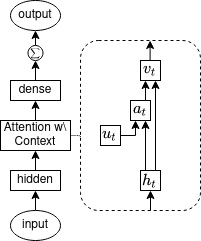
\includegraphics[width=0.35\linewidth]{II_Body/LSTM/images/AttenrionDrawing.png}
    \caption{Attention based architecture}
    \label{fig:attention}
\end{figure}
\begin{equation}
    \begin{split}
        \hat{u_t} &= tanh \left(W h_{t} + b \right) \\
             \alpha_t &= \frac{exp(u^T u)}{\sum_t(exp(u_t^T u))} \\
              v_t &= \alpha_t*h_t, v in time t
    \end{split}
    \label{eq:AttentionWithContext}
\end{equation}
\begin{equation}
    \begin{split}
        v = \sum_t(\alpha_t * h_t)
    \end{split}
    \label{eq:Addition}
\end{equation}

% \subsection{Implementation}
%     Following table higlighs parameters, which provided best results for their experements.
%     \textbf{Table of the parameters.}
%     The network will be the one discussed above.
%     Model itself will be multi-feature based with follwoing parameters: Voltage \textit{V(t)}, Current \textit{A(t)} and Temperature \textit{C(t)}, where \textit{t} represents a time-stamp. Each feature will contain equal amount of sample and each will be feed in input column vector. As a result, a single input will have following form: \\
%     % [V(0)], [I(0)], [T(0)] \\
%     % [V(1)], [I(1)], [T(1)] \\
%     % [V(n)], [I(n)], [T(n)] \\
%     where \textit{n} is the history size.
%     The output vector will be a State of Charge \textit{SoC(\%)} percentage up to 2 decimal places, within range 0 to 1 and time stamp \textit{n}: \\
%     % [SoC(n)] \\
%     As a result the shape of input and output data will be: X(0)=(n,3) and Y(0)=(1)
%     The entire dataset will use single-step windowing tecnhinue with no bathces to save memory and utilsase \textbf{stateless}* \footnote{Need to discuss this with Holmes.} model. \\
%     The Generated dataset of sample size \textit{k}, will consist of two Tensor input/output Vectors of following shape: \\
%     X = (k-n,n,3), Y = (k-n,1).
%     The variable type for computation was selected to be float32.
%     To keep Denerated dataset simple, no batching approach spared from dealing with 4-dimensional input vectors.
% \subsection{Prediction results}


%     Implementation of the model based on Chemali2017. Application for our section and results. Refer to methodology from time to time.